\documentclass[a4paper]{article}
\usepackage{ucs}  % unicode
\usepackage[utf8x]{inputenc}
% \usepackage[T2A]{fontenc}
% \usepackage[bulgarian]{babel}
\usepackage{graphicx}
% \usepackage{fancyhdr}
% \usepackage{lastpage}
\usepackage{listings}
\usepackage{slashbox}
\usepackage{multirow}
\usepackage{wrapfig}
\usepackage{amsfonts}
\usepackage{amsmath, amsthm, amssymb}
% \usepackage{fancyvrb}
% \usepackage[usenames,dvipsnames]{color}
% \setlength{\headheight}{12.51453pt}

%\pagestyle{fancy}
%\fancyhead{}
%\fancyfoot{}

% \cfoot{\thepage\ от \pageref{LastPage}}

% \addto\captionsbulgarian{%
%   \def\abstractname{%
%     Цел на проекта} %\cyr\CYRA\cyrs\cyrt\cyrr\cyra\cyrk\cyrt}}%
% }

% Custom defines:
\def\definition{Definition:\ }
\def\la{\leftarrow}
\def\vars{\mathrm{Vars}}
\def\occ{\mathrm{Occ}}
\def\lub{\sqcup}
\def\xlub{\underline\lub}
\def\glb{\sqcap}
% \def\dc{bar baz}

% TODO remove colorlinks before printing
% \usepackage[unicode,colorlinks]{hyperref}   % this has to be the _last_ command in the preambule, or else - no work
% \hypersetup{urlcolor=blue}
% \hypersetup{citecolor=PineGreen}

\begin{document}

\newcommand{\aee}[1] {[[#1]]^\sharp}
\newcommand{\cc}[1] {\texttt{#1}}
\def\A {\mathcal{A}}
\def\N {\mathcal{N}}
\def\NonZero {\mathrm{NonZero}}
\def\Zero {\mathrm{Zero}}
\def\Vars {\mathrm{Vars}}
\def\Occ {\mathrm{Occ}}

\title{Static Program Analysis - Exercise 5}
\author{Iskren Ivov Chernev \\ tutorial group B}

\maketitle

\section{Solution}

\begin{tabular}{|c|l|}
\hline
\multicolumn{2}{|c|}{Iteration 1} \\
\hline
0 & $ (-\infty, +\infty) $                                                          \\
1 & $ \bot \lub ([0, 0] \lub \bot) = [0, 0] $                                       \\
2 & $ \bot \lub ([0, 0] \glb (-\infty, 41]) = [0, 0] $                              \\
3 & $ \bot \xlub ([0, 0] \glb [0, 41]) = [0, 0] $                                   \\
4 & $ \bot \lub [0, 0] = [0, 0] $                                                   \\
5 & $ \bot \lub [0, 0] = [0, 0] $                                                   \\
6 & $ \bot \lub [1, 1] = [1, 1] $                                                   \\
7 & $ \bot $                                                                        \\
8 & $ \bot $                                                                        \\
\hline
\multicolumn{2}{|c|}{Iteration 2} \\
\hline
0 & $ (-\infty, +\infty) $                                                          \\
1 & $ [0, 0] \lub ([0, 0] \lub [1, 1]) = [0, 1] $                                   \\
2 & $ [0, 0] \lub ([0, 1] \glb (-\infty, 41]) = [0, 1] $                            \\
3 & $ [0, 0] \xlub ([0, 1] \glb [0, 41]) = [0, 0] \xlub [0, 1] = [0, +\infty) $     \\
4 & $ [0, 0] \lub [0, +\infty) = [0, +\infty) $                                     \\
5 & $ [0, 0] \lub [0, +\infty) = [0, +\infty) $                                     \\
6 & $ [1, 1] \lub [1, +\infty) = [1, +\infty) $                                     \\
7 & $ \bot $                                                                        \\
8 & $ \bot $                                                                        \\
\hline
\multicolumn{2}{|c|}{Iteration 3} \\
\hline
0 & $ (-\infty, +\infty) $                                                          \\
1 & $ [0, 1] \lub ([0, 0] \lub [1, +\infty)) = [0, +\infty) $                       \\
2 & $ [0, 1] \lub ([0, +\infty) \glb (-\infty, 41]) = [0, 41] $                     \\
3 & $ [0, +\infty) \xlub ([0, 41] \glb [0, 41]) = [0, +\infty) $                    \\
4 & $ [0, +\infty) \lub [0, +\infty) = [0, +\infty) $                               \\
5 & $ [0, +\infty) \lub [0, +\infty) = [0, +\infty) $                               \\
6 & $ [1, +\infty) \lub [1, +\infty) = [1, +\infty) $                               \\
7 & $ \bot $                                                                        \\
8 & $ \bot \lub ([0, +\infty) \glb [42, +\infty)) = [42, +\infty) $                 \\
\hline

\end{tabular}

We don't get the exact value of $ i $ at program point $ 8 $, but optimize out $ 7 $.

\section{Solution}

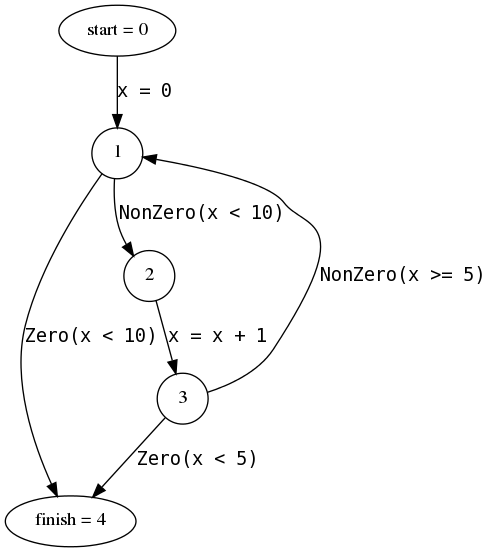
\includegraphics[scale=0.3]{5-2.png}

This program shows that naive narrowing is more precise than accelerated
narrowing. It is easy to see that on the naive widening will calculate $ [0,
+\infty) $ at position 2 on the second iteration. Accelerated narrowing will
use the condition $ \NonZero(x < 10) $ to calculate $ [0, 9] $ at position 2 in
the first iteration. However on the second one from position 3 the updated
bound $ [1, 4] $ won't be merged into 2, because only one change from infinity
to non infinity is permitted. Thus position 2 will remain $ [0, 9] $, while the
naive narrowing will produce the correct result $ [0, 4] $ for position 2 on
the second iteration.

\section{Solution}

The factorial program with interval analysis is an example of this. We just
need to add an unaccessible node (no in/out edges). Whitelist is faster than
round-robin, because round-robin requires one iteration to realize it has
finished. The recursive algorithm outperform whitelist because the unaccessible
node won't be calculated in the recursion, because it won't be required for the
computations (because it is unaccessible). The whitelist will calculate it
once, because all nodes are inserted in the list initially.

\end{document}
